\documentclass{scrartcl}

\usepackage{amsmath}
\usepackage{amssymb}
\usepackage{dsfont}
\usepackage[utf8]{inputenc}
\usepackage[T1]{fontenc}
\usepackage{csquotes}
\usepackage{graphicx}
\usepackage{hyperref}
\usepackage{hypcap}
\usepackage{mathrsfs}
\usepackage{tikz}

\usepackage[backend=biber, style=numeric]{biblatex}
\addbibresource{bib/thesis_refs.bib}

\title{Confinement in SU(2) gauge theory on a lattice}
\subtitle{A numerical study}
\date{December 2022}
\author{Heinrich von Campe}

\begin{document}
\maketitle

\begin{abstract}
In this very short review, we present (i) the Metropolis algorithm which is
a method of approximately solving path integrals and (ii) the Wilson formalism,
a formulation of (in our case) an SU(2) gauge theory on a lattice. By applying
the former to the latter, we study the distance dependence of the static potential
of a quark antiquark pair. Confinement is demonstrated with this.
\end{abstract}

\section{Introduction}
Confinement is a very interesting feature of non-abelian gauge theories:
E.\,g. in Quantum Chromodynamics (an SU(3) gauge theory), there cannot be any
free quarks, they only appear in bound states. By studying the potential of a
static quark antiquark pair, one may try to find an indication of this: If the
potential displays a \emph{linear} dependence on the distance between quark and
antiquark, this indicates confinement.

Unfortunately, QCDs running coupling with large values of the coupling for low
momenta makes it impossible to study this problem pertubatively. Therefore, one
has to resort to non-analytical methods. In our case, the lattice formulation
of a non-abelian gauge theory (SU(2), for simplicity, not QCD) was chosen.

This is a short summary of a longer thesis on the topic~\cite{thesis}, it is
organised as follows: In section \ref{sec:markov}, the numerical algorithm used to
attack the problem is presented. Then, in section \ref{sec:wilson}, we present the
formulation of the gauge theory that is suited for simulations. Finally, in
section \ref{sec:confinement}, we present the results of the numerical studies
and, in sec. \ref{sec:conclusion}, we discuss possible further topics
of study.

\section{Markov} \label{sec:markov}
Markov Chain Monte Carlo (MCMC) algorithms allow to numerically approximate
path integrals such as~\cite{freedmanCreutz}
\[
    \langle O \rangle = \frac{1}{Z} \int \mathscr{D} [x] O[x] e^{-S[x]},
    \; Z = \int \mathscr{D} [x] e^{-S[x]}.
\]
The interpretation is thus: $x$ represents a single trajectory, the measure
$\mathscr{D}[x]$ means that all possible trajectories are integrated over. $O$ is
an observable whose expectation value one is interested in. It is calculated by
evaluating it at the different $x$ where the trajectories are weighted by
$\frac{1}{Z}e^{-S[x]}$. $S$ is the action and the path integral is
evaluated at $\hbar = 1$ and Euclidian time. Thus just the minus sign in front of it and not the
imaginary unit.~\footnote{This has the positive side effect that the numerical
calculations become much easier given that one has to deal with exponentially
supressed factors insted of oscillating phases.}
Here, $Z$ accounts for the normalisation of the integral. It is suggestively named:
As one may see, MCMC algorithms may be used equally to numerically compute
canonical partition sums from statistical mechanics.

The basic idea of these algorithm is to draw many samples
$\sim \frac{1}{Z} e^{-S[x]}$ and then to approximate the expectation
value $\langle O \rangle$ by the arithmetic mean $\overline{O}$ of the observable
evaluated at the  different samples. For MCMC, this is realised by the generation
of multiple generations of configurations $\{x\}$ where $W(x,x')$ describes the
probability of passing from configuration $x$ to $x'$. When applied repeatedly,
the samples will eventually follow the right distribution if, and only if, the
\emph{detailed balance} condition is met:~\cite{freedmanCreutz}
\[
    \frac{W(x,x')}{W(x',x)} = \frac{e^{-S[x']}}{e^{-S[x]}} =: e^{-\Delta S[x',x]}.
\]
A very simple algorithm that meets this criterion is that of \emph{Metropolis}
which works as follows: Given a configuration $x$, a new configuration $x'$ is
generated at random. This new configuration will be accepted with probability
~\cite{freedmanCreutz}
\begin{equation} \label{eq:metropolis}
W(x,x') = \begin{cases}
    1, &\text{if } \Delta S < 0,\\
    e^{-\Delta S}, &\text{else}.
\end{cases}
\end{equation}

\section{Wilson} \label{sec:wilson}
Having established a tool to calculate path integrals given the classical action,
we now turn to the question of finding a formulation of an action for an SU(2)
gauge theory that is appropriate for simulations. In the continuous case, the action
describing the gauge field $A(x)$ is the one of Yang and Mills:~\cite{gattringerLang}
\[
    S_\text{YM} [A] = \frac{1}{2g^2} \int \text{d}^4 x \, \
        \text{tr} [F_{\mu \nu}(x) F^{\mu \nu}(x)],
    \; F_{\mu \nu} = \frac{1}{i} [D_\mu, D_\nu] \
    = \partial_\mu A_\nu - \partial_\nu A + i [A_\mu, A_\nu],
\]
where the trace is taking over the colour indices.

Due to finite memory and computing time, one can only simulate a discretised
version of the gauge field. Instead of (Euclidian) space time $\mathbb{R}^4$, a
\emph{lattice} $\Lambda$ of discrete points is studied.~\footnote{Technically,
the lattice is actually a \emph{torus} with periodic boundary conditions.}
On the lattice, the gauge field \enquote{lives} on the links between the points.
~\footnote{This is contrary to e.\,g. a bosonic field which will \enquote{live}
on the lattice points.}
The variables are named $U_\mu(x) \in \text{SU(2)}$~\footnote{The links are elements
are elements of the gauge group contrary to the gauge field, which are elements
of the algebra.} where $\mu$ denotes the direction
towards which the link points starting at the point $x$. With these, one may formulate
the \emph{Wilson} action~\cite{urbachCPscript}
\begin{equation} \label{eq:wilson}
    S_\text{W} = \frac{\beta}{2} \sum_{x \in \Lambda} \sum_{\mu < \nu} \
    \text{Re tr } [\mathds{1} - U_{\mu \nu}(x)], \; \beta = \frac{4}{g^2}.
\end{equation}
The \emph{plaquette} describes a square of the gauge links:
%\[
%U_{\mu \nu} (x) = U_\mu(x) U_\nu(x + a\hat{\mu}) U^\dag_\mu(x + a\hat{\nu}) U^\dag_\nu(x).
%\]
\[
U_{\mu \nu}(x) =
\begin{tikzpicture}[baseline=-0.5ex]
\draw[->, red, very thick] (0,-.5) -> (1,-.5);
\draw[->, blue, very thick] (1,-.5) -> (1,.5);
\draw[->, orange, very thick] (1,.5) -> (0,.5);
\draw[->, brown, very thick] (0,.5) -> (0,-.5);
\foreach \x in {0,...,1}
{
	\foreach \y in {-.5,...,.5}
	{
		\fill[color=black] (\x,\y) circle (.04);
	}
}
\end{tikzpicture}
= \textcolor{red}{U_\mu(x)}
\textcolor{blue}{U_\nu(x + a_\mu)}
\textcolor{orange}{U_\mu(x + a_\nu)^\dag}
\textcolor{brown}{U_\nu(x)^\dag}.
\]		
Here, $\hat{\mu}$ is a basis vector in direction $\mu$ and $a$ is the lattice spacing.
(So, $U_\mu(x)$ points from lattice site $x$ in direction $\mu$,
$U_\nu(x + a \hat{\mu}$) points from there in direction $\nu$ etc. as illustrated
above.)
One may demonstrate that, in the continuum limit, the Wilson action approaches
the one of Yang and Mills, $S_\text{W} \xrightarrow{a\rightarrow 0} S_\text{YM}$.
~\cite{gattringerLang}
Opposed to a naive discretisation, the Wilsonian approach has the advantage of
retaining gauge invariance. A nice way of looking at the two actions is as follows:
The fact that the field strength tensor may be calculated as the commutator of the
covariant derivatives signifies that the Yang Mills action measures \emph{curvature}.
The Wilson action does the equivalent on the lattice by summing all those squares of
link variables. Indeed, with the definition of the link variables as the path
ordered integral of the gauge field, one may recover the limit mentioned above.

As an observable of this system, we consider the perhaps most simple possible
composition of the lattice variables: rectangles. These are generalisations of the
plaquettes $U_{\mu \nu}$ and could be written like
$W(r,t) = \text{tr} \; \prod_{x \in \mathcal{C}} U(x)$.
Here, $r$ denotes the extend of the rectangle $\mathcal{C}$ in time direction and $r$
the extend in one of the spacial directions of the lattice. One may show that
the expectation value of these \emph{Wilson loops} approximately scale like
~\cite{loopsStaticPotRothe}
\begin{equation} \label{eq:wilsonLoop}
    \langle W(r,t) \rangle \sim e^{-t V(r)}
\end{equation}
for large values of $t$. Here, $V(r)$ is the potential of a static quark antiquark
pair. Thus, by studying the system described above, one could indeed draw conclusions
about how such a quark antiquark potential $V$ scales with the distance $r$.

\section{Confinement} \label{sec:confinement}
The simulation carried out was in principle quite simple: A lattice is set up,
where on each of the lattice links an SU(2) matrix is saved. Using the Wilson
action \eqref{eq:wilson}, the Metropolis algorithm \eqref{eq:metropolis} is
employed to generate lattice configurations. The action is measured after each
iteration. Once its value stabilises, the measurements can start. Now, Wilson
loops of different sizes are measured with breaks of several iterations (several
to reduce correlation between the measurements).

\begin{figure}[htpb]
    \centering
    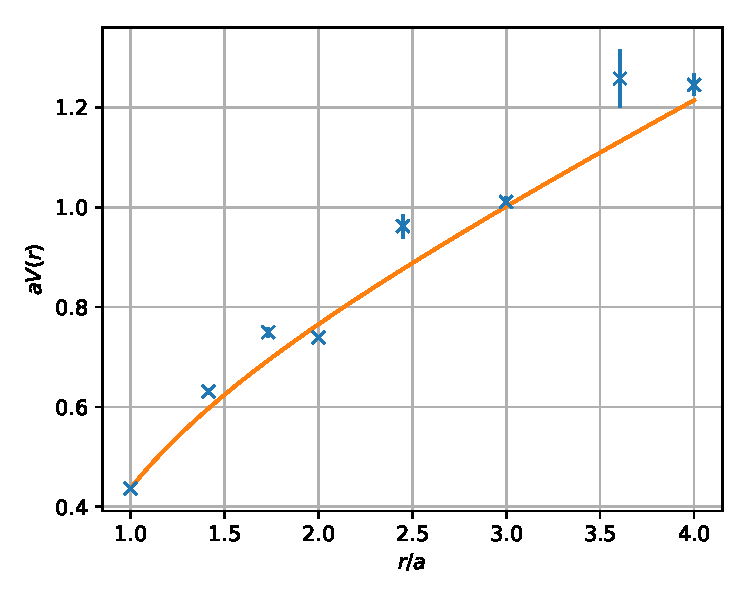
\includegraphics[width=0.8\textwidth]{figs/aVfitBeta23}
    \caption{The static potential dep. on the distance $r$ between quark and
    antiquark (measured in units of lattice spacing $a$). The non-integer values
    of $r$ stem from measurements of non planar Wilson loops. A linear dependence
    is clearly visible.}
    \label{fig:aVfit}
\end{figure}

At fixed $r$, several measurements of $\overline{W(r,t)}$ allow to extract the
value of $V(r)$ by using \eqref{eq:wilsonLoop}. The results are plotted in
figure \ref{fig:aVfit}. The most prominent feature of this graph is the fact
that there is a linear component of the potential. This indicates confinement:
In order to pull apart a quark antiquark pair, one needs to invest more and more
as the distance between the two grows. This is a very prominent feature of
non-abelian gauge theories. If we had studied an abelian gauge theory, the
behaviour of the potential would be purely Coulomb like, without the linear
component.

\section{Conclusion} \label{sec:conclusion}
We have succesfully demonstrated the appearance of confinement in an SU(2) lattice
gauge theory. There are several possible further points of interest, both on the
technical and physical side: One might want to improve the estimation of the
uncertainty of the estimator of the expectation values. Furthermore, one could
study a larger lattice to get more data points and more samples to reduce the
uncertainty.

More interestingly, one might want to study SU(3) which bears actual physical
relevance for it is realised in nature. However, this would be much more complicated 
than the SU(2) case since one would actually need to exponentiate the generators to
get elements of the group. (For SU(2), this could be circumvented by exploiting
that SU(2) $\cong S^3$.) On the other hand, it would be feasible to study
U(1), an  \emph{abelian} gauge theory. Here, one would expect no confinement.

Finally, it should again be noted that this is but a brief summary of a short
thesis on this topic. For more details concerning the Metropolis algorithm, we
refer to \cite{freedmanCreutz} and for the Wilson formalism
\cite{gattringerLang} and \cite{loopsStaticPotRothe} may be recommended.
\printbibliography
\end{document}
